% figures/ch03-dimension-chart.tex
% Chapter 5: dimensions of cusp forms for SL_2(Z)
\begin{figure}[ht]
\centering
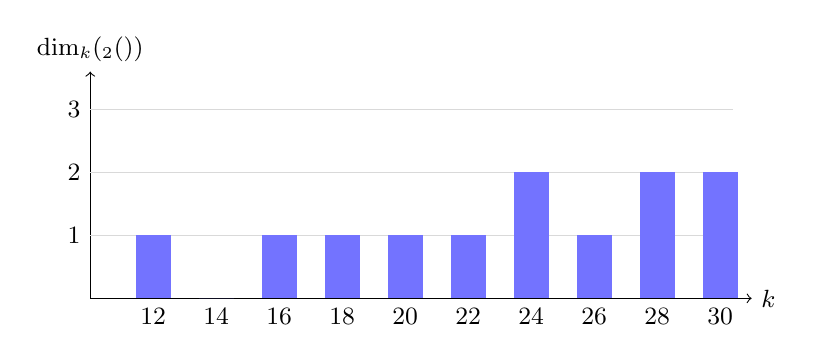
\begin{tikzpicture}[x=0.8cm,y=0.8cm,font=\small]
  \draw[->] (0,0) -- (10.5,0) node[right] {$k$};
  \draw[->] (0,0) -- (0,3.6) node[above] {$\dim \Sk_k(\SL_2(\Z))$};

  \foreach \x/\k in {1/12,2/14,3/16,4/18,5/20,6/22,7/24,8/26,9/28,10/30}
    \node[below] at (\x,0) {\k};

  \foreach \y in {1,2,3}
    {\draw[gray!30] (0,\y) -- (10.2,\y); \node[left] at (0,\y) {\y};}

  \foreach \x/\h in {1/1,2/0,3/1,4/1,5/1,6/1,7/2,8/1,9/2,10/2}
    \fill[blue!55] (\x-0.28,0) rectangle (\x+0.28,\h);
\end{tikzpicture}
\caption{$\SL_2(\Z)$ 上尖点形式空间维数的前几个值。最早出现的非零空间是 $\Sk_{12}=\C\Delta$；之后维数按“每跨过一个 $12$ 就大致增加 $1$”的节奏增长。}
\label{fig:dimension-chart}
\end{figure}
